\documentclass[a4paper,12pt]{article}

\sloppy
\frenchspacing

\usepackage[left=4cm,top=4cm,right=4cm,bottom=4cm,nohead]{geometry}
\usepackage[utf8]{inputenc}
\usepackage[magyar]{babel}
\usepackage{listings}
\usepackage{multicol}
\usepackage{graphicx}
\usepackage{float}

\title{Szoftverarchitektúrák (VIAUM105)\\Egyszerű verziókövető rendszer\\Rendszerterv}
\author{Vajna Miklós (AYU9RZ)\\Veres-Szentkirályi András (YZIOAW)}

\begin{document}

\maketitle
\thispagestyle{empty}
\lstset{numbers=left, numberstyle=\tiny, basicstyle=\ttfamily, breaklines=true, frame=single, tabsize=2}

\pagebreak
\onehalfspacing
\section{Bevezetés}

Jelen rendszerterv célja a házi feladat tervezése során meghozott döntések
dokumentálása. A döntéseket két csoportra oszthatjuk:

\begin{itemize}
\item architektúrával kapcsolatos döntések
\item az egyes rétegekkel kapcsolatos döntések
\end{itemize}

\section{Architektúra}

A rendszert 3 réteg alkotja:

\begin{figure}[H]
\centering
\includegraphics[width=25mm,keepaspectratio]{layers.pdf}
\caption{A verziókövető rendszer architektúrája}
\end{figure}

\begin{itemize}
\item Adatbázis réteg: SQL adatbázis az entitások permanens tárolására.
\item Kiszolgáló: itt kerül implementálásra az üzleti logika, tehát minden
olyan funkcionalitás, mely nem triviális, és megjelenítés-független.
\item Kliens: a megjelenítési rétegért felel, csak triviális funkciókat
tartalmaz, minden egyéb funkciót a kiszolgálón keresztül biztosít.
\end{itemize}

\clearpage
\section{Adatbázis réteg}

Fizikailag a következő entitásokat kívánunk tárolni:

\begin{itemize}
\item a rendszer felhasználóit
\item a modelleket
\item a modellek egyes verzióit
\item a modellekhez való hozzáférési jogokat
\end{itemize}

\begin{figure}[H]
\centering
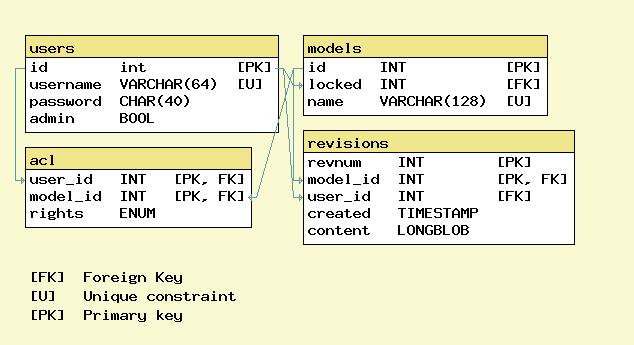
\includegraphics[width=120mm,keepaspectratio]{sqlschema.png}
\caption{Az adatbázis sémájának modellje}
\end{figure}

Az ábrán látható módon ezek között a következő kapcsolatokat tervezzük:

\begin{itemize}
\item a felhasználók és modellek között jogosultságokat adhatunk meg
\item a felhasználók zárolhatják a modelleket
\item a modellekhez egy-egy felhasználó verziókat hozhat létre
\end{itemize}

\clearpage
\section{Üzleti logika}

Az üzleti logika lefelé az adatbázis felé SQL segítségével kommunikál, a
megjelenítési réteg felé pedig CORBA interfészeken.

Az interfészek:

\begin{figure}[H]
\centering
\includegraphics[width=130mm,keepaspectratio]{classdiagram.pdf}
\caption{Az adatbázis sémájának modellje}
\end{figure}

\clearpage
Az interfészek tervezésekor látszólagos problémát jelentett, hogy az
interfészek öröklődése is megengedett (amihez aztán az omniORB csonk
osztályokat generál), valamint mi is örököltetni akartuk az ilyen interfészek
egyes implementációit.

Példa erre a User és a UserAdmin osztályok. Ebben az esetben a UserAdmin
egyrészt a POA\_VersionControl:: UserAdmin osztályból kellene öröklődjön,
másrészt viszont az UserImpl implementációs osztályban már megvalósított
logikát szeretnénk újrahasznosítani. Ezt úgy oldottuk meg, hogy ténylegesen a
UserImpl osztályt adtuk meg ősnek, viszont a kliens egy UserAdminImpl
osztállyal paraméterezett POA\_VersionControl:: UserAdmin\_tie osztályt kapott
vissza, amely a UserAdmin interfészből öröklődik.

Az üzleti logika tervezésekor ezen kívül még két döntést hoztunk az alkalmazás
biztoságának növelése érdekében:

\begin{itemize}
\item A kliensek csak az Auth interfészhez férnek hozzá, és ezen keresztül érik
el hitelesítés után a többi interfészt.
\item Az SQL parancsok végrehajtásakor kizárólag prepared statementek
segítségével helyettesítünk be paramétereket, ezáltal elkerülve az esetleges
SQL injection problémakörébe tartozó veszélyeket.
\end{itemize}

A megvalósítás során, utólag hoztuk a döntést, hogy idő hiányában a 3-way merge
funkcionalitást egy külső, szabadon elérhető (LGPL) könyvtár segítségével
oldjuk meg. Mivel a kiválasztott LibXDiff könyvtár C nyelven íródott, az
előadáson ismertetett Wrapper Facade tervezési mintát használva készítettük el
a Resolver interfészt a könyvtár általunk használni kívánt részéhez.

\section{Megjelenítési réteg}

FIXME

\section{Befejezés}

A rétegek áttekintése után nem maradt más hátra, mint áttekinteni, hogy milyen
módszert terveztünk használni a szoftver teszteléséhez. A specifikációnak
megfelelően automatikus tesztelést az üzleti logikára valósítottuk meg.

A teszt keretrendszert a cppunit projekt adja. A tesztek futtatása előtt a
CORBA szervert automatikusan indítjuk, kapcsolódunk egy külön erre a célra
allokált teszt adatbázishoz. Minden interfészt egy külön teszt osztály tesztel,
az adatbázist minden teszt előtt inicializáljuk. A teszt végén bontjuk a
kapcsolatot a teszt-adatbázissal, valamint leállítjuk a CORBA szervert.

\section{Továbbfejlesztési lehetőségek}

A rendszer elkészítése során több továbbfejlesztési lehetőség is eszünkbe
jutott, melyeket idő hiányában még nem tudtunk megvalósítani:

\begin{itemize}
\item Az omniORB alapértelmezetten nem támogatja az SSL használatát a CORBA
kommunikáció során. Jelenleg erre megoldásként a VPN használatát tudjuk
javasolni, ennek ellenére lenne értelme mind a kliens, mind az szerver esetén
beállíthatóvá tenni az SSL-t, arra az esetre ha mégis mindkét oldalon elérhető
lenne az omniORB SSL támogatása.
\item A jelenleg 3-way merge kód általában szöveges állományok merge-ölésére
lett kifejlesztve, ezt le lehetne cserélni egy olyan algoritmusra, ami
specifikusan SQL scriptek kezelésére készült, ezáltal növelve az automatikusan
feloldható ütközések arányát.
\item A Qt-alapú kliens mellett webes felületet is lehetne készíteni a
rendszerhez.
\end{itemize}

\end{document}
